\documentclass{../praktikum-protokollvorlage-latex/include/protokollclassE}
\SelectLanguage{english}

\newcommand{\praktikum}{P3}
\newcommand{\semester}{WS17/18}

\newcommand{\wochentag}{Mo}
\newcommand{\gruppennr}{XX}

\newcommand{\nachnamea}{Elicabuk}
\newcommand{\vornamea}{Umut}
\newcommand{\nachnameb}{Pittermann}
\newcommand{\vornameb}{Martin}

\input{../common/emails.tex}

\hyphenation
{
	über-nom-me-nen
	an-ge-ge-be-nen
}

\newcommand{\maketitlepage}
{
	\begingroup \let\clearpage\relax
	\tableofcontents
	\listoffigures
	\listoftables
	\endgroup
}

\newcommand{\configureappendix}
{
	\chapter*{\appendixname} \addcontentsline{toc}{chapter}{\appendixname}
}

\newcommand{\s}[1]{\ensuremath{_\text{#1}}}


\newcommand{\versuch}{Angle Correlation}
\newcommand{\versuchsnr}{106}			%P!- weglassen

\newcommand{\betreuer}{Dick Butt}
\newcommand{\durchgefuehrt}{23.10.2017}

\newcommand{\abstract}{\ce{^{60}Co} decays by beta decay to the activated isotope \ce{^{60}Ni}. The activated nickel nucleus emits two gamma rays of energies \SI{1.17}{\MeV} and \SI{1.33}{\MeV}. Theory suggests that the successive gamma emissions must be distributed anisotropically. The angular correlation function and resolution time of coincidences are determined.} %The abstract
\begin{document}
	\FrontMatter
	% coordinates for background border
\newcommand{\diameter}{20}
\newcommand{\xone}{-15}
\newcommand{\xtwo}{160}
\newcommand{\yone}{15}
\newcommand{\ytwo}{-253}

\newcommand{\hoehea}{60}
\newcommand{\hoeheb}{60}




\begin{titlepage}
    % background border
    \begin{tikzpicture}[overlay]
    \draw[color=gray]
            (\xone mm, \yone mm)
      -- (\xtwo mm, \yone mm)
    arc (90:0:\diameter pt)
      -- (\xtwo mm + \diameter pt , \ytwo mm)
        -- (\xone mm + \diameter pt , \ytwo mm)
    arc (270:180:\diameter pt)
        -- (\xone mm, \yone mm);
    \end{tikzpicture}

    % KIT logo
    \begin{textblock}{10}[0,0](4.5,2.5)
        \includegraphics[width=.25\textwidth]{../praktikum-protokollvorlage-latex/include/kitlogo.pdf}
    \end{textblock}
    \changefont{phv}{m}{n}    % helvetica
    \begin{textblock}{10}[0,0](5.5,2.2)
        \begin{flushright}
            \Large FAKULTÄT FÜR PHYSIK\\Praktikum Klassische Physik
        \end{flushright}
    \end{textblock}

    \begin{textblock}{10}[0,0](4.2,3.1)
        \begin{tikzpicture}[overlay]
        \draw[color=gray]
            (\xone mm + 5 mm, -12 mm)
         -- (\xtwo mm + \diameter pt - 5 mm, -12 mm);
        \end{tikzpicture}
    \end{textblock}

    \Large
    % Zeile 1
    \begin{textblock}{12}[0,0](3.58,4.4)
        \mytextfield{Prak.}{\praktikum}{0.9cm}{17pt}
                    {P1/P2}{2}{Praktikum}
    \end{textblock}
    \begin{textblock}{12}[0,0](5.53,4.4)
        \mytextfield{Semester}{\semester}{2.6cm}{17pt}
        {z.B. \glqq WS14/15\grqq\ oder \glqq SS15\grqq}{0}{Semester}
    \end{textblock}
    \begin{textblock}{12}[0,0](9.53,4.4)
        \mytextfield{Wochentag}{\wochentag}{1.3cm}{17pt}
                    {Mo/Di/Mi/Do}{2}{Wochentag}
    \end{textblock}
    \begin{textblock}{12}[0,0](12.88,4.4)
       \mytextfield{Gruppennr.}{\gruppennr}{1.06cm}{17pt}
                   {\#\#}{2}{Gruppennummer}
    \end{textblock}

    % Zeile 2
    \begin{textblock}{12}[0,0](3.58,4.95)
        \mytextfield{Name}{\nachnamea}{6cm}{17pt}
                    {}{0}{Name1}
    \end{textblock}
    \begin{textblock}{12}[0,0](9.53,4.95)
        \mytextfield{Vorname}{\vornamea}{6cm}{17pt}
                    {}{0}{Vorname1}
    \end{textblock}

    % Zeile 3
    \begin{textblock}{12}[0,0](3.58,5.5)
        \mytextfield{Name}{\nachnameb}{6cm}{17pt}
                    {}{0}{Name2}
    \end{textblock}
    \begin{textblock}{12}[0,0](9.53,5.5)
        \mytextfield{Vorname}{\vornameb}{6cm}{17pt}
                    {}{0}{Vorname2}
    \end{textblock}

    % Zeile 4
    \begin{textblock}{12}[0,0](3.64,6.05)
       \normalsize\mytextfield{Emailadresse(n)}{\emailadressen}{13.1cm}{10pt}
                              {Optional}{0}{Emailadressen}
    \end{textblock}

    % Zeile 5
    \begin{textblock}{12}[0,0](3.58,7)
        \mytextfield{Versuch}{\versuch\ (\praktikum-\versuchsnr)}{9.45cm}{14pt}
                    {z.B. \glqq Galvanometer (P1-13)\grqq\ oder \glqq %
                     Mikrowellenoptik (P2-15)\grqq}{0}{Versuch}
    \end{textblock}

    % Zeile 6
    \begin{textblock}{12}[0,0](3.58,7.55)
        \mytextfield{Betreuer}{\betreuer}{7cm}{17pt}{}{0}{Betreuer}
    \end{textblock}
    \begin{textblock}{12}[0,0](10.82,7.55)
        \mytextfield{Durchgeführt am}{\durchgefuehrt}{2.53cm}{17pt}
                    {TT.MM.JJ}{8}{Durchfuehrung}
    \end{textblock}

    % Querstrich
    \begin{textblock}{20}[0,0](0,7.9)\tiny\centering
        Wird vom Betreuer ausgefüllt.
    \end{textblock}
    \begin{tikzpicture}[overlay]
    \draw[color=gray]
        (\xone mm + 5 mm, -95 mm)
     -- (\xtwo mm + \diameter pt - 5 mm, -95 mm);
    \end{tikzpicture}

    % Zeile 1
    \begin{textblock}{12}[0,0](3.65,8.57)
        \myTtextfield{1. Abgabe am}{}{2.5cm}{17pt}
                     {}
    \end{textblock}

    % Block 1
    \begin{tikzpicture}[overlay]
    \draw[color=gray]
        (\xone mm + 10 mm, -107.5 mm)
     -- (\xtwo mm + \diameter pt - 10 mm, -107.5 mm)
     -- (\xtwo mm + \diameter pt - 10 mm, -107.5 mm - \hoehea mm)
     -- (\xone mm + 10 mm, -107.5 mm - \hoehea mm)
     -- (\xone mm + 10 mm, -107.5 mm);
    \end{tikzpicture}
    \begin{textblock}{20}[0,0](3.8,9.2)
        \myTtextfield{Rückgabe am}{}{2.5cm}{17pt}
                     {}
    \end{textblock}
    \begin{textblock}{20}[0,0](8.7,9.2)
        \smash{Begründung:}
    \end{textblock}

    % Zeile 2
    \begin{textblock}{12}[0,0](3.65,12.6)
        \myTtextfield{2. Abgabe am}{}{2.5cm}{17pt}
                     {}
    \end{textblock}

    % Block 2
    \begin{tikzpicture}[overlay]
    \draw[color=gray]
        (\xone mm + 10 mm, -180 mm)
     -- (\xtwo mm + \diameter pt - 10 mm, -180 mm)
     -- (\xtwo mm + \diameter pt - 10 mm, -180 mm - \hoehea mm)
     -- (\xone mm + 10 mm, -180 mm - \hoehea mm)
     -- (\xone mm + 10 mm, -180 mm);
    \end{tikzpicture}
    \begin{textblock}{12}[0,0](4,13.25)
        \smash{Ergebnis:~~~~+~~~/~~~0~~~/~~~-}
    \end{textblock}
    \begin{textblock}{12}[0,0](9.5,13.25)
        \smash{Fehlerrechnung:~~~Ja~~~/~~~Nein}
    \end{textblock}
    \begin{textblock}{12}[0,0](3.8,13.72)
        \myTtextfield{Datum}{}{2.5cm}{17pt}
                     {}
    \end{textblock}
    \begin{textblock}{12}[0,0](8.3,13.72)
        \myTtextfield{Handzeichen}{}{5.5cm}{17pt}
                     {}
    \end{textblock}
    \begin{textblock}{12}[0,0](4,14.25)\Large
        \smash{Bemerkungen:}
    \end{textblock}



    % lowest text blocks concerning the KIT
    \begin{textblock}{10}[0,0](4,16.8)
        \tiny{KIT -- Universität des Landes Baden-Württemberg und nationales %
              Forschungszentrum in der Helmholtz-Gemeinschaft}
    \end{textblock}
    \begin{textblock}{10}[0,0](14,16.75)
        \large{\textbf{www.kit.edu}}
    \end{textblock}
\end{titlepage}

	\maketitlepage

	\MainMatter

	\chapter{Introduction}

\section{Correlation Function}
\begin{figure}[tbp]
	\centering
	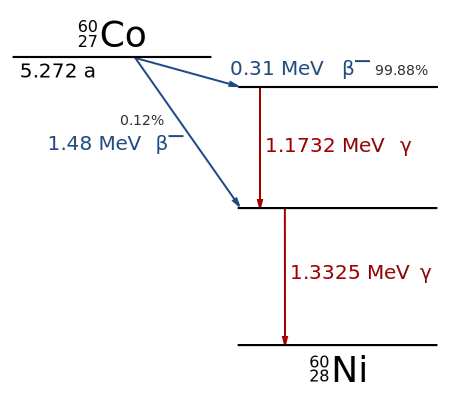
\includegraphics[width=.3\textwidth]{./img/co60_decay.pdf}
	\caption*{Source: \url{commons.wikimedia.org/wiki/File:Cobalt-60_Decay_Scheme.svg}}
	\caption[The decay cascade of \ce{^{60}Co}]{\textbf{The decay cascade of \ce{^{60}Co}} After decaying from a 5+ spin state to a 4+ spin state of \ce{^{60}Ni} by beta decay with a probability of \num{99.88}\%, two gamma rays of energies \SI{1.17}{\MeV} and \SI{1.33}{\MeV} are emitted, each inhibting a spin of 2+.}
	\label{fig:co60_cascade}
\end{figure}
When the nucleus emits two gamma rays in a cascade, as shown in \autoref{fig:co60_cascade}, the spatial angular distribution of the second photon with respect to the first photon's direction of travel is anisotropic.
In particular, by detecting two rays of a cascade simultaneously, the equal population of states is removed, resulting in an anisotropy of the second ray's angular distribution.
The relative probability of the gamma ray's emission at an angle $\theta$ relative to the first photon is denoted as $W(\theta)$.
Normalizing this differential cross-section at $\theta=\SI{90}{\degree}$ yields the correlation function

\begin{equation*}
	K(\theta) = 1 + \sum_{k}^{k_\text{max}}a_{2k}\cdot\cos^{2k}{\theta}.
\end{equation*}

The series terminates at $k_\text{max}=\min(I, L_1, L_2)=2$, where $I, L_1, L_2$ denote the nuclear spin after the first gamma emission and the angular momenta of both gamma rays respectively.
This results in the correlation function

\begin{equation}\label{eq:corr_func}
	K(\theta) = 1 + a_2\cos^{2}{\theta} + a_4\cos^{4}{\theta},
\end{equation}
while only pure multipole orders (quadrupoles) are assumed.

The deviation of a correlation function from an isotropic angular distribution is called \textbf{anisotropy}
\begin{equation}\label{eq:aniso}
	An=\frac{K(180)-K(90)}{K(90)}=K(180)-1
\end{equation}

\section{Resolution Time}
Utilizing the relation
\begin{equation}\label{eq:res_time}
	\tau_\text{res}=\frac{N_\text{R}}{N_1\cdot N_2}\cdot T,
\end{equation}
where $N_\text{R}$ denotes random event count, $N_{1/2}$ the number of events of channel 1/2 respectively and $T$ the length of the measurement, the resolution time of coincidences can be computed. \todo{Kinda bloated sentence. Any suggestions?}

\section{Detectors}
To not only being able to detect the mere presence of a gamma ray but also its energy, two \ce{NaI}-scintillators doped with \ce{Th} are employed.
Sodium iodide is an inorganic scintillator crystal and grants the advantage of most of the gamma rays being observed through the photoelectric effect.
Coupled to these scintillator crystals are two photomultiplier stages that output a voltage proportional to the incoming gamma ray's energy. \todo{Is it? i.e. non-linearity of crystals}
The output is digitized for later analysis.


	%\Appendix
\configureappendix

	%\TheBibliography
\bibliographystyle{babalpha}
\bibliography{../common/lit}

\end{document}
